% $Header$

\documentclass{beamer}

% This file is a solution template for:

% - Talk at a conference/colloquium.
% - Talk length is about 20min.
% - Style is ornate.



% Copyright 2004 by Till Tantau <tantau@users.sourceforge.net>.
%
% In principle, this file can be redistributed and/or modified under
% the terms of the GNU Public License, version 2.
%
% However, this file is supposed to be a template to be modified
% for your own needs. For this reason, if you use this file as a
% template and not specifically distribute it as part of a another
% package/program, I grant the extra permission to freely copy and
% modify this file as you see fit and even to delete this copyright
% notice.


\mode<presentation>
{
  \usetheme{Warsaw}
  % or ...

  \setbeamercovered{transparent}
  % or whatever (possibly just delete it)
}


\usepackage[english]{babel}
% or whatever

\usepackage[latin1]{inputenc}
% or whatever

\usepackage{times}
\usepackage[T1]{fontenc}
% Or whatever. Note that the encoding and the font should match. If T1
% does not look nice, try deleting the line with the fontenc.




\usepackage{listings}
\usepackage{color}

\definecolor{dkgreen}{rgb}{0,0.6,0}
\definecolor{gray}{rgb}{0.5,0.5,0.5}
\definecolor{mauve}{rgb}{0.58,0,0.82}

\lstset{frame=tb,
  language=C++,
  aboveskip=3mm,
  belowskip=3mm,
  breaklines=true,
  breakatwhitespace=true,
  basicstyle={\footnotesize\ttfamily},
  showstringspaces=false,
  columns=flexible,
  numbers=left,
  numberstyle=\tiny\color{gray},
  keywordstyle=\color{blue},
  commentstyle=\color{dkgreen},
  stringstyle=\color{mauve},
  emphstyle={\color{blue}\textbf},
  tabsize=4
}

\usepackage[ruled, vlined, noend, procnumbered]{algorithm2e}




\usepackage{tikz}
\usepgflibrary{arrows.meta}
\usetikzlibrary{arrows.meta}
% \usetikzlibrary{graphs}





% {n1/n3, n2/n3, n2/n4,n4/n3, n4/n5,n5/n2, n5/n6, n6/n3, n6/n4}
% {n1/n2}
\newcommand{\mygrapha}[3]{
	\begin{tikzpicture}
		[scale=.5,auto=left,every node/.style={circle,draw,semithick,fill=blue!20,radius=0.4}]
		\node (n2) at (1,5)	{2};
		\node (n5) at (2,1)	{5};
		\node (n1) at (4,7)	{1};
		\node (n4) at (4,3)	{4};
		\node (n6) at (6,1)	{6};
		\node (n3) at (7,5)	{3};

		% black edge
		\foreach \from/\to in #1
			\draw [black, thick, -{Stealth[length=2mm]}] (\from) -- (\to);
		% red edge
		\foreach \from/\to in #2
			\draw [red, thick, -{Stealth[length=2mm]}] (\from) -- (\to);
		#3
	\end{tikzpicture}
}





\title[Path-based DFS] % (optional, use only with long paper titles)
{Path-based depth-first search for strong and biconnected components}

\author[Harold N. Gabow] % (optional, use only with lots of authors)
{\textbf{Author of the paper: Harold N. Gabow}\newline\newline
 {Reported by: T.T. Liu \and D.P. Xu \and B.Y. Chen } }
% - Give the names in the same order as the appear in the paper.
% - Use the \inst{?} command only if the authors have different
%   affiliation.

\date{\scriptsize{\today} }

\subject{Algorithms}
% This is only inserted into the PDF information catalog. Can be left
% out.



% If you have a file called "university-logo-filename.xxx", where xxx
% is a graphic format that can be processed by latex or pdflatex,
% resp., then you can add a logo as follows:

\pgfdeclareimage[height=0.75cm]{university-logo}{sdulogo}
\logo{\pgfuseimage{university-logo}}



% Delete this, if you do not want the table of contents to pop up at
% the beginning of each subsection:
\AtBeginSubsection[]
{
  \begin{frame}<beamer>{Outline}
    \tableofcontents[currentsection,currentsubsection]
  \end{frame}
}


% If you wish to uncover everything in a step-wise fashion, uncomment
% the following command:

%\beamerdefaultoverlayspecification{<+->}


\begin{document}





\defverbatim[colored]\mycodea{%
\begin{lstlisting}[frame=single, emph={P, v, v_k, v_i, w, G, H}, 
deletekeywords={new, and, in, to, not, of, set, delete}, morekeywords={end, end if}]
H = G;
while H still has a vertex v
	start a new path P = (v);
	while P is not empty
		if the last vertex v_k of P has an edge (v_k, w)
			if w belongs to P
				contract the cycle v_i(w), ... , v_k, both in H and in P; /* w and v_i are identical. */
			else
				add w to P, as the new last vertex of P;
			end if
\end{lstlisting}
}

\defverbatim[colored]\mycodeb{%
\begin{lstlisting}[frame=single, emph={P, v, v_k, v_i, w, G, H},
firstnumber=last, deletekeywords={new, and, in, to, not, of, set, delete}, morekeywords={end, end if}]
		else
			output v_k as a vertex of the strong component graph;
			delete v_k from both H and P;
		end if
	end
end
\end{lstlisting}
}

\defverbatim[colored]\mycodec{%
\begin{lstlisting}[frame=single, emph={P, v, v_k, v_i, w, G, H}, 
firstnumber=7, deletekeywords={new, and, in, to, not, of, set, delete}, morekeywords={end, end if}]
contract the cycle v_i(w), ... , v_k, both in H and in P; /* w and v_i are identical. */
\end{lstlisting}
}

% \defverbatim[colored]\mycoded{%
% \begin{lstlisting}[frame=single, emph={G,S,B,v,I,c,n}]
% }





\begin{frame}
  \titlepage
\end{frame}

\begin{frame}{Outline}
  \tableofcontents
  % You might wish to add the option [pausesections]
\end{frame}


% Structuring a talk is a difficult task and the following structure
% may not be suitable. Here are some rules that apply for this
% solution:

% - Exactly two or three sections (other than the summary).
% - At *most* three subsections per section.
% - Talk about 30s to 2min per frame. So there should be between about
%   15 and 30 frames, all told.

% - A conference audience is likely to know very little of what you
%   are going to talk about. So *simplify*!
% - In a 20min talk, getting the main ideas across is hard
%   enough. Leave out details, even if it means being less precise than
%   you think necessary.
% - If you omit details that are vital to the proof/implementation,
%   just say so once. Everybody will be happy with that.

\section{Introduction}

\begin{frame}{Several Questions}
	\begin{itemize}
		\item
		One-pass or two-pass?
		\item
		LOWPOINT?
		\item
		Ear decomposition?
		\item
		Compele version?
		\item
		Robbin's Theorem?
	\end{itemize}
\end{frame}

\section{Strong Components}

\subsection{Thinking about Strong Components}


\begin{frame}{Review: What have we learned from the textbook?}{Concepts of Strong Components}
	\begin{itemize}
		\item
		Two \alert{mutually reachable} vertices are in the same \emph{strong component}.
	\end{itemize}
	\begin{exampleblock}{Example}
	\begin{center}
	\mygrapha{{n1/n2, n1/n3, n2/n3, n2/n4,n4/n3, n4/n5,n5/n2, n5/n6, n6/n3, n6/n4}}{{}}{
		\fill [yellow, semitransparent] (1,0) -- (0,5) -- (1,7) -- (8,0) -- cycle;
		\fill [yellow, semitransparent] (3,6) rectangle (5,8);
		\fill [yellow, semitransparent] (6,4) rectangle (8,6);
	}
	\end{center}
	\end{exampleblock}
\end{frame}

\begin{frame}{Review: What have we learned from the textbook?}{Algorithms to Find Strong Components}
	\begin{itemize}
		\item
		Idea: Run DFS twice. Once on the original graph $G$, once on the \emph{tranposition} of $G^T$.
		\item
		Trick: Using \emph{finishing times} of each vertex computed by the first DFS.
		\item
		Linear time complexity: $O(V+E)$
	\end{itemize}
\end{frame}


\subsection{Purdom and Munro's high-level algorithm}
% This high-level algorithm was originally proposed by Purdom and Munro, mentioned after the pseudo-code in the paper.

\begin{frame}{Pseudo-Code}%[fragile]
	\mycodea
	\begin{itemize}
		\item
		Note that \emph{contracting} means selecting one vertex as a representation and \alert{merging} others rather than deleting them.
	\end{itemize}
\end{frame}

\begin{frame}{Pseudo-Code (Continued)}%[fragile]
	\mycodeb
\end{frame}

\begin{frame}{Assessment}
	\begin{itemize}
		\item
		The time consumption of each statement in the pseudo-code is clear. Total time complexity is linear.
		except the statement in line 7:
	\end{itemize}
	\mycodec
	\begin{itemize}
		\item
		Problem is how to merge in linear time while keeping the next time accessing this vertex still in constant time.
		\item
		Therefore, a good data structure for disjoint set merging is needed.
	\end{itemize}
\end{frame}

\begin{frame}{Examples}
	\begin{columns}
		\begin{column}{5.5cm}
			\begin{exampleblock}{Block B}
				The second line. \newline
				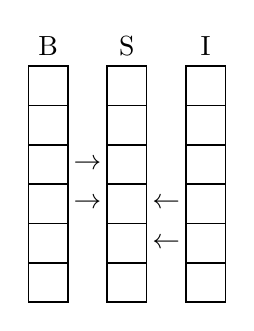
\begin{tikzpicture}
					[scale=.5,auto=left]
					% text
					\draw node at (0.5, 0.5) {B};
					\draw node at (2.5, 0.5) {S};
					\draw node at (4.5, 0.5) {I};
					% grid					
					\foreach \x in {0,-1,-2,-3,-4,-5} {
						\draw [semithick] (0, \x) rectangle (1,\x-1);
						\draw [semithick] (2, \x) rectangle (3,\x-1);
						\draw [semithick] (4, \x) rectangle (5,\x-1);
					}
					% rightarrow
					\foreach \x in {-2, -3}
						\draw node at (1.5, \x-0.5) {$\rightarrow$};
					% leftarrow
					\foreach \x in {-3, -4}
						\draw node at (3.5, \x-0.5) {$\leftarrow$};
				\end{tikzpicture}
			\end{exampleblock}
		\end{column}
		\begin{column}{5.5cm}
			\begin{exampleblock}{Block C}
				The third line. \newline
			\end{exampleblock}
		\end{column}
	\end{columns}
\end{frame}


\subsection{Contribution}

\begin{frame}{His Contribution}%{Subtitles are optional.}
  % - A title should summarize the slide in an understandable fashion
  %   for anyone how does not follow everything on the slide itself.

	\begin{itemize}
		\item
		He gave a simple list-based implementation that achieves linear time.
		\item
		Use only stacks and arrays as data structure. % Mentioned in introduction.
		% Do not need a disjoint set merging data structure.
	\end{itemize}
\end{frame}

\begin{frame}[fragile]{New algorithm to discover strong components}
	\begin{procedure}[H]
		\small
		\caption{STRONG(G)}
		empty stacks S and B\;
		\For{$v\in V$}{
			$I[v]=0$\;
		}
		$c=n$\;
		\For{$v\in V$}{
			\If{$I[v]=0$}{
				DFS($v$)\;
			}
		}
	\end{procedure}
\end{frame}

\begin{frame}[fragile]{New algorithm to discover strong components}
	\begin{procedure}[H]
		\scriptsize
		\caption{DFS(v)}
		PUSH(v,S);\quad I[v]$=$TOP(S);\quad PUSH(I[v],B)\;
		\tcc{add v to the end of P}
		\For{egdes$(v,w)\in E$}{
			\uIf{$I[v]=0$}{
				DFS(w)\;
			}\Else(\tcc*[h]{contract if necessary}){
				\While{$I[w]<B[TOP[B]]$}{POP(B)\;}
			}
			\If{$I[v]=B[TOP(B)]$} {
				\tcc{number vertices of the next strong component}
				POP(B)\;
				increase c by 1\;
				\While{$I[v]\leq TOP[S]$}{I[POP(S)]$=$c\;}
			}
		}
	\end{procedure}
\end{frame}

\section*{Summary}

\begin{frame}{Summary}

  % Keep the summary *very short*.
  \begin{itemize}
  \item
    The \alert{first main message} of your talk in one or two lines.
  \item
    The \alert{second main message} of your talk in one or two lines.
  \item
    Perhaps a \alert{third message}, but not more than that.
  \end{itemize}

  % The following outlook is optional.
  \vskip0pt plus.5fill
  \begin{itemize}
  \item
    Outlook
    \begin{itemize}
    \item
      Something you haven't solved.
    \item
      Something else you haven't solved.
    \end{itemize}
  \end{itemize}
\end{frame}



% All of the following is optional and typically not needed.
\appendix
\section<presentation>*{\appendixname}
\subsection<presentation>*{For Further Reading}

\begin{frame}[allowframebreaks]
  \frametitle<presentation>{For Further Reading}

  \begin{thebibliography}{10}

  \beamertemplatebookbibitems
  % Start with overview books.

  \bibitem{Author1990}
    A.~Author.
    \newblock {\em Handbook of Everything}.
    \newblock Some Press, 1990.


  \beamertemplatearticlebibitems
  % Followed by interesting articles. Keep the list short.

  \bibitem{Someone2000}
    S.~Someone.
    \newblock On this and that.
    \newblock {\em Journal of This and That}, 2(1):50--100,
    2000.
  \end{thebibliography}
\end{frame}

\end{document}


